\documentclass[12pt]{article}
\usepackage[utf8]{inputenc}
\usepackage[T1]{fontenc}
\usepackage{pdflscape} 
\usepackage{lmodern}
\usepackage[a4paper,bindingoffset=0.2in,%
            left=0.5in,right=0.5in,top=0.5in,bottom=1in,%
            footskip=.25in]{geometry}
\usepackage[colorlinks=true, linkcolor=Black, urlcolor=Blue]{hyperref}
\usepackage{graphicx}
\usepackage{subcaption}
\usepackage{listings}
\usepackage{color}
\usepackage[table]{xcolor}
\definecolor{lightgray}{gray}{0.9}

\definecolor{codegreen}{rgb}{0,0.6,0}
\definecolor{codegray}{rgb}{0.5,0.5,0.5}
\definecolor{codepurple}{rgb}{0.58,0,0.82}
\definecolor{backcolour}{rgb}{0.95,0.95,0.92}

\lstdefinestyle{mystyle}{
	backgroundcolor=\color{backcolour},   
	commentstyle=\color{codegreen},
	keywordstyle=\color{magenta},
	numberstyle=\tiny\color{codegray},
	stringstyle=\color{codepurple},
	basicstyle=\ttfamily\footnotesize,
	breakatwhitespace=false,         
	breaklines=true,                 
	captionpos=b,                    
	keepspaces=true,                 
	numbers=left,                    
	numbersep=5pt,                  
	showspaces=false,                
	showstringspaces=false,
	showtabs=false,                  
	tabsize=2
}


\begin{document}
\title{Projekt - Drzewa Decyzyjne II\\
\large Sebastian Michoń 136770, Marcin Zatorski 136834\\
\large grupe L5}
\date{\vspace{-10ex}}
\maketitle

\section{Wybrane najważniejsze atrybuty}
\begin{enumerate}
	\item sex - nawet jeśli płeć sama w sobie może nie być dobrze skorelowana z tym, czy student zdał, wpływa ona na to, jak dany atrybut wpływa na studenta - np. dla mężczyzn wyższą korelację z wynikiem końcowym może mieć chęć podjęcia edukacji wyższej raczej niż zdrowie, dla kobiet - wręcz przeciwnie.
	
	\item reason - to, dlaczego student wybrał daną szkołę.
	\item failures
	\item higher
	\item Dalc - dzienne spożycie alkoholu w dni robocze
	\item health
	\item absences	
\end{enumerate}

\section{Wybrane metryki}
\begin{enumerate}
	\item Accuracy - jako, że dataset jest dosyć zrównoważony (115/85 dla zestawu treningowego i 118/77 dla testowego) wykorzystanie procentu trafień jest zasadne.
	\item F1 measure - jeśli jakaś inna miara poza celnością jest zasadna, to najprędzej F1 - pozwala ona bowiem zagregować informację o precyzji i czułości
	\item Ostatnią miarą, która zostanie użyta jest Balanced accuracy - \(\frac{TPR+TNR}{2}\), czyli suma czułości i selektywności podzielona przez przez 2 - nieco lepsza niż Accuracy, jako że proporcja w tym datasecie to 3:2 (gdzie więcej osób nie zdało niż zdało)
\end{enumerate}

\begin{flushleft}
		\rowcolors{2}{gray!25}{white}
		\captionof{table}{Wyniki algorytmu J48 dla wybranych atrybutów - Math dataset}
		\scalebox{0.65}{
			\begin{tabular}{| l | l | l | l | l | l | l | l | l | l | l | l | l | l | l | l | l | l | l | l | l |}
				\rowcolor{gray!50}
				\hline
				Binary Split & Confidence factor & Minimum objects & TP & FP & FN & TN & Accuracy & F1 & Balanced Accuracy\\ \hline
				0 & 0.1000 & 2 & 31 & 37 & 46 & 81 & 0.5744 & 0.4276 & 0.5445\\ \hline
				0 & 0.2000 & 2 & 31 & 37 & 46 & 81 & 0.5744 & 0.4276 & 0.5445\\ \hline
				0 & 0.3000 & 2 & 31 & 37 & 46 & 81 & 0.5744 & 0.4276 & 0.5445\\ \hline
				0 & 0.4000 & 2 & 31 & 37 & 46 & 81 & 0.5744 & 0.4276 & 0.5445\\ \hline
				0 & 0.5000 & 2 & 27 & 28 & 50 & 90 & 0.6000 & 0.4091 & 0.5567\\ \hline
				0 & 0.6000 & 2 & 28 & 35 & 49 & 83 & 0.5692 & 0.4000 & 0.5335\\ \hline
				0 & 0.7000 & 2 & 28 & 35 & 49 & 83 & 0.5692 & 0.4000 & 0.5335\\ \hline
				0 & 0.8000 & 2 & 28 & 35 & 49 & 83 & 0.5692 & 0.4000 & 0.5335\\ \hline
				0 & 0.9000 & 2 & 28 & 35 & 49 & 83 & 0.5692 & 0.4000 & 0.5335\\ \hline
				1 & 0.1000 & 2 & 31 & 37 & 46 & 81 & 0.5744 & 0.4276 & 0.5445\\ \hline
				1 & 0.2000 & 2 & 31 & 37 & 46 & 81 & 0.5744 & 0.4276 & 0.5445\\ \hline
				1 & 0.3000 & 2 & 27 & 29 & 50 & 89 & 0.5949 & 0.4060 & 0.5524\\ \hline
				1 & 0.4000 & 2 & 26 & 23 & 51 & 95 & 0.6205 & 0.4127 & 0.5714\\ \hline
				1 & 0.5000 & 2 & 26 & 23 & 51 & 95 & 0.6205 & 0.4127 & 0.5714\\ \hline
				1 & 0.6000 & 2 & 30 & 30 & 47 & 88 & 0.6051 & 0.4380 & 0.5677\\ \hline
				1 & 0.7000 & 2 & 30 & 30 & 47 & 88 & 0.6051 & 0.4380 & 0.5677\\ \hline
				1 & 0.8000 & 2 & 30 & 30 & 47 & 88 & 0.6051 & 0.4380 & 0.5677\\ \hline
				1 & 0.9000 & 2 & 30 & 30 & 47 & 88 & 0.6051 & 0.4380 & 0.5677\\ \hline
				0 & 0.1000 & 3 & 31 & 37 & 46 & 81 & 0.5744 & 0.4276 & 0.5445\\ \hline
				0 & 0.2000 & 3 & 31 & 37 & 46 & 81 & 0.5744 & 0.4276 & 0.5445\\ \hline
				0 & 0.3000 & 3 & 31 & 37 & 46 & 81 & 0.5744 & 0.4276 & 0.5445\\ \hline
				0 & 0.4000 & 3 & 31 & 37 & 46 & 81 & 0.5744 & 0.4276 & 0.5445\\ \hline
				0 & 0.5000 & 3 & 23 & 27 & 54 & 91 & 0.5846 & 0.3622 & 0.5349\\ \hline
				0 & 0.6000 & 3 & 24 & 34 & 53 & 84 & 0.5538 & 0.3556 & 0.5118\\ \hline
				0 & 0.7000 & 3 & 24 & 34 & 53 & 84 & 0.5538 & 0.3556 & 0.5118\\ \hline
				0 & 0.8000 & 3 & 24 & 34 & 53 & 84 & 0.5538 & 0.3556 & 0.5118\\ \hline
				0 & 0.9000 & 3 & 24 & 34 & 53 & 84 & 0.5538 & 0.3556 & 0.5118\\ \hline
				1 & 0.1000 & 3 & 31 & 37 & 46 & 81 & 0.5744 & 0.4276 & 0.5445\\ \hline
				1 & 0.2000 & 3 & 31 & 37 & 46 & 81 & 0.5744 & 0.4276 & 0.5445\\ \hline
				1 & 0.3000 & 3 & 31 & 37 & 46 & 81 & 0.5744 & 0.4276 & 0.5445\\ \hline
				1 & 0.4000 & 3 & 25 & 29 & 52 & 89 & 0.5846 & 0.3817 & 0.5395\\ \hline
				1 & 0.5000 & 3 & 25 & 25 & 52 & 93 & 0.6051 & 0.3937 & 0.5564\\ \hline
				1 & 0.6000 & 3 & 28 & 28 & 49 & 90 & 0.6051 & 0.4211 & 0.5632\\ \hline
				1 & 0.7000 & 3 & 28 & 28 & 49 & 90 & 0.6051 & 0.4211 & 0.5632\\ \hline
				1 & 0.8000 & 3 & 28 & 28 & 49 & 90 & 0.6051 & 0.4211 & 0.5632\\ \hline
				1 & 0.9000 & 3 & 28 & 28 & 49 & 90 & 0.6051 & 0.4211 & 0.5632\\ \hline
				0 & 0.1000 & 4 & 31 & 37 & 46 & 81 & 0.5744 & 0.4276 & 0.5445\\ \hline
				0 & 0.2000 & 4 & 31 & 37 & 46 & 81 & 0.5744 & 0.4276 & 0.5445\\ \hline
				0 & 0.3000 & 4 & 31 & 37 & 46 & 81 & 0.5744 & 0.4276 & 0.5445\\ \hline
				0 & 0.4000 & 4 & 31 & 37 & 46 & 81 & 0.5744 & 0.4276 & 0.5445\\ \hline
				0 & 0.5000 & 4 & 31 & 37 & 46 & 81 & 0.5744 & 0.4276 & 0.5445\\ \hline
				0 & 0.6000 & 4 & 25 & 27 & 52 & 91 & 0.5949 & 0.3876 & 0.5479\\ \hline
				0 & 0.7000 & 4 & 25 & 27 & 52 & 91 & 0.5949 & 0.3876 & 0.5479\\ \hline
				0 & 0.8000 & 4 & 25 & 27 & 52 & 91 & 0.5949 & 0.3876 & 0.5479\\ \hline
				0 & 0.9000 & 4 & 25 & 27 & 52 & 91 & 0.5949 & 0.3876 & 0.5479\\ \hline
				1 & 0.1000 & 4 & 31 & 37 & 46 & 81 & 0.5744 & 0.4276 & 0.5445\\ \hline
				1 & 0.2000 & 4 & 31 & 37 & 46 & 81 & 0.5744 & 0.4276 & 0.5445\\ \hline
				1 & 0.3000 & 4 & 25 & 28 & 52 & 90 & 0.5897 & 0.3846 & 0.5437\\ \hline
				1 & 0.4000 & 4 & 25 & 28 & 52 & 90 & 0.5897 & 0.3846 & 0.5437\\ \hline
				1 & 0.5000 & 4 & 25 & 24 & 52 & 94 & 0.6103 & 0.3968 & 0.5606\\ \hline
				1 & 0.6000 & 4 & 25 & 24 & 52 & 94 & 0.6103 & 0.3968 & 0.5606\\ \hline
				1 & 0.7000 & 4 & 25 & 24 & 52 & 94 & 0.6103 & 0.3968 & 0.5606\\ \hline
				1 & 0.8000 & 4 & 25 & 24 & 52 & 94 & 0.6103 & 0.3968 & 0.5606\\ \hline
				1 & 0.9000 & 4 & 25 & 24 & 52 & 94 & 0.6103 & 0.3968 & 0.5606\\ \hline
				0 & 0.1000 & 5 & 40 & 53 & 37 & 65 & 0.5385 & 0.4706 & 0.5352\\ \hline
				0 & 0.2000 & 5 & 19 & 16 & 58 & 102 & 0.6205 & 0.3393 & 0.5556\\ \hline
				0 & 0.3000 & 5 & 19 & 16 & 58 & 102 & 0.6205 & 0.3393 & 0.5556\\ \hline
				0 & 0.4000 & 5 & 19 & 16 & 58 & 102 & 0.6205 & 0.3393 & 0.5556\\ \hline
				0 & 0.5000 & 5 & 19 & 16 & 58 & 102 & 0.6205 & 0.3393 & 0.5556\\ \hline
				0 & 0.6000 & 5 & 19 & 16 & 58 & 102 & 0.6205 & 0.3393 & 0.5556\\ \hline
				0 & 0.7000 & 5 & 19 & 16 & 58 & 102 & 0.6205 & 0.3393 & 0.5556\\ \hline
				0 & 0.8000 & 5 & 19 & 16 & 58 & 102 & 0.6205 & 0.3393 & 0.5556\\ \hline
				0 & 0.9000 & 5 & 19 & 16 & 58 & 102 & 0.6205 & 0.3393 & 0.5556\\ \hline
				1 & 0.1000 & 5 & 36 & 49 & 41 & 69 & 0.5385 & 0.4444 & 0.5261\\ \hline
				1 & 0.2000 & 5 & 22 & 18 & 55 & 100 & 0.6256 & 0.3761 & 0.5666\\ \hline
				1 & 0.3000 & 5 & 24 & 27 & 53 & 91 & 0.5897 & 0.3750 & 0.5414\\ \hline
				1 & 0.4000 & 5 & 24 & 27 & 53 & 91 & 0.5897 & 0.3750 & 0.5414\\ \hline
				1 & 0.5000 & 5 & 24 & 27 & 53 & 91 & 0.5897 & 0.3750 & 0.5414\\ \hline
				1 & 0.6000 & 5 & 24 & 27 & 53 & 91 & 0.5897 & 0.3750 & 0.5414\\ \hline
				1 & 0.7000 & 5 & 24 & 27 & 53 & 91 & 0.5897 & 0.3750 & 0.5414\\ \hline
				1 & 0.8000 & 5 & 24 & 27 & 53 & 91 & 0.5897 & 0.3750 & 0.5414\\ \hline
				1 & 0.9000 & 5 & 24 & 27 & 53 & 91 & 0.5897 & 0.3750 & 0.5414\\ \hline
				
			\end{tabular}
	}\end{flushleft}

\clearpage
\section{Działanie algorytmu - Generowane drzewa}
\begin{figure}[h!]
	\subsection{Dyskretny Age}
	\centering
	\begin{subfigure}[b]{1\linewidth}
		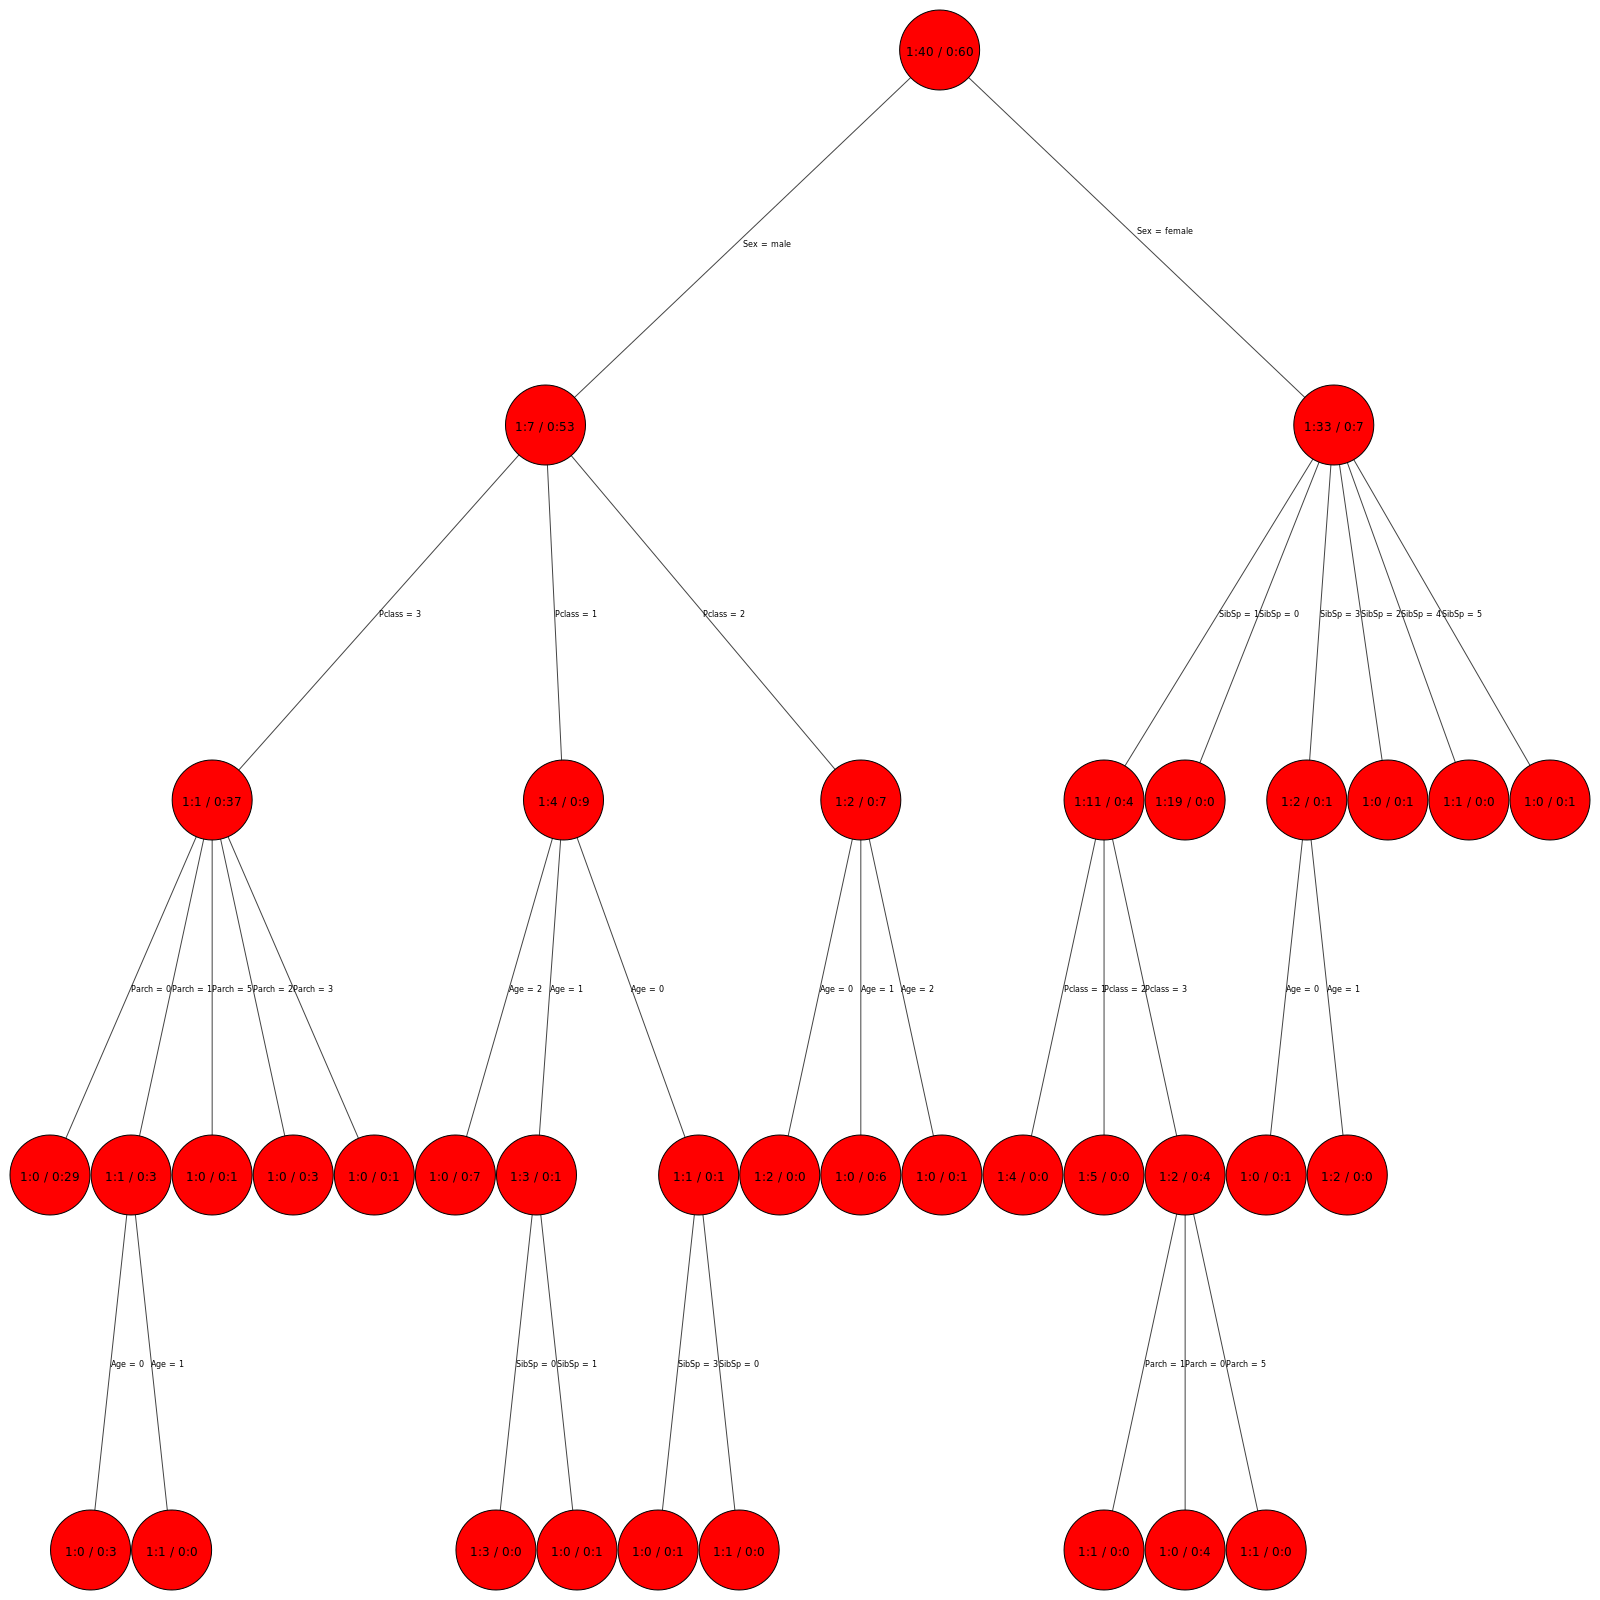
\includegraphics[width=\linewidth]{Dyskretny.png}
	\end{subfigure}
	\label{fig:dyskretne}
	\caption{Age jest atrybutem dyskretnym}
\end{figure}


\clearpage
\begin{figure}[h!]
	\subsection{Ciągły Age}
	\centering
	\begin{subfigure}[b]{1\linewidth}
		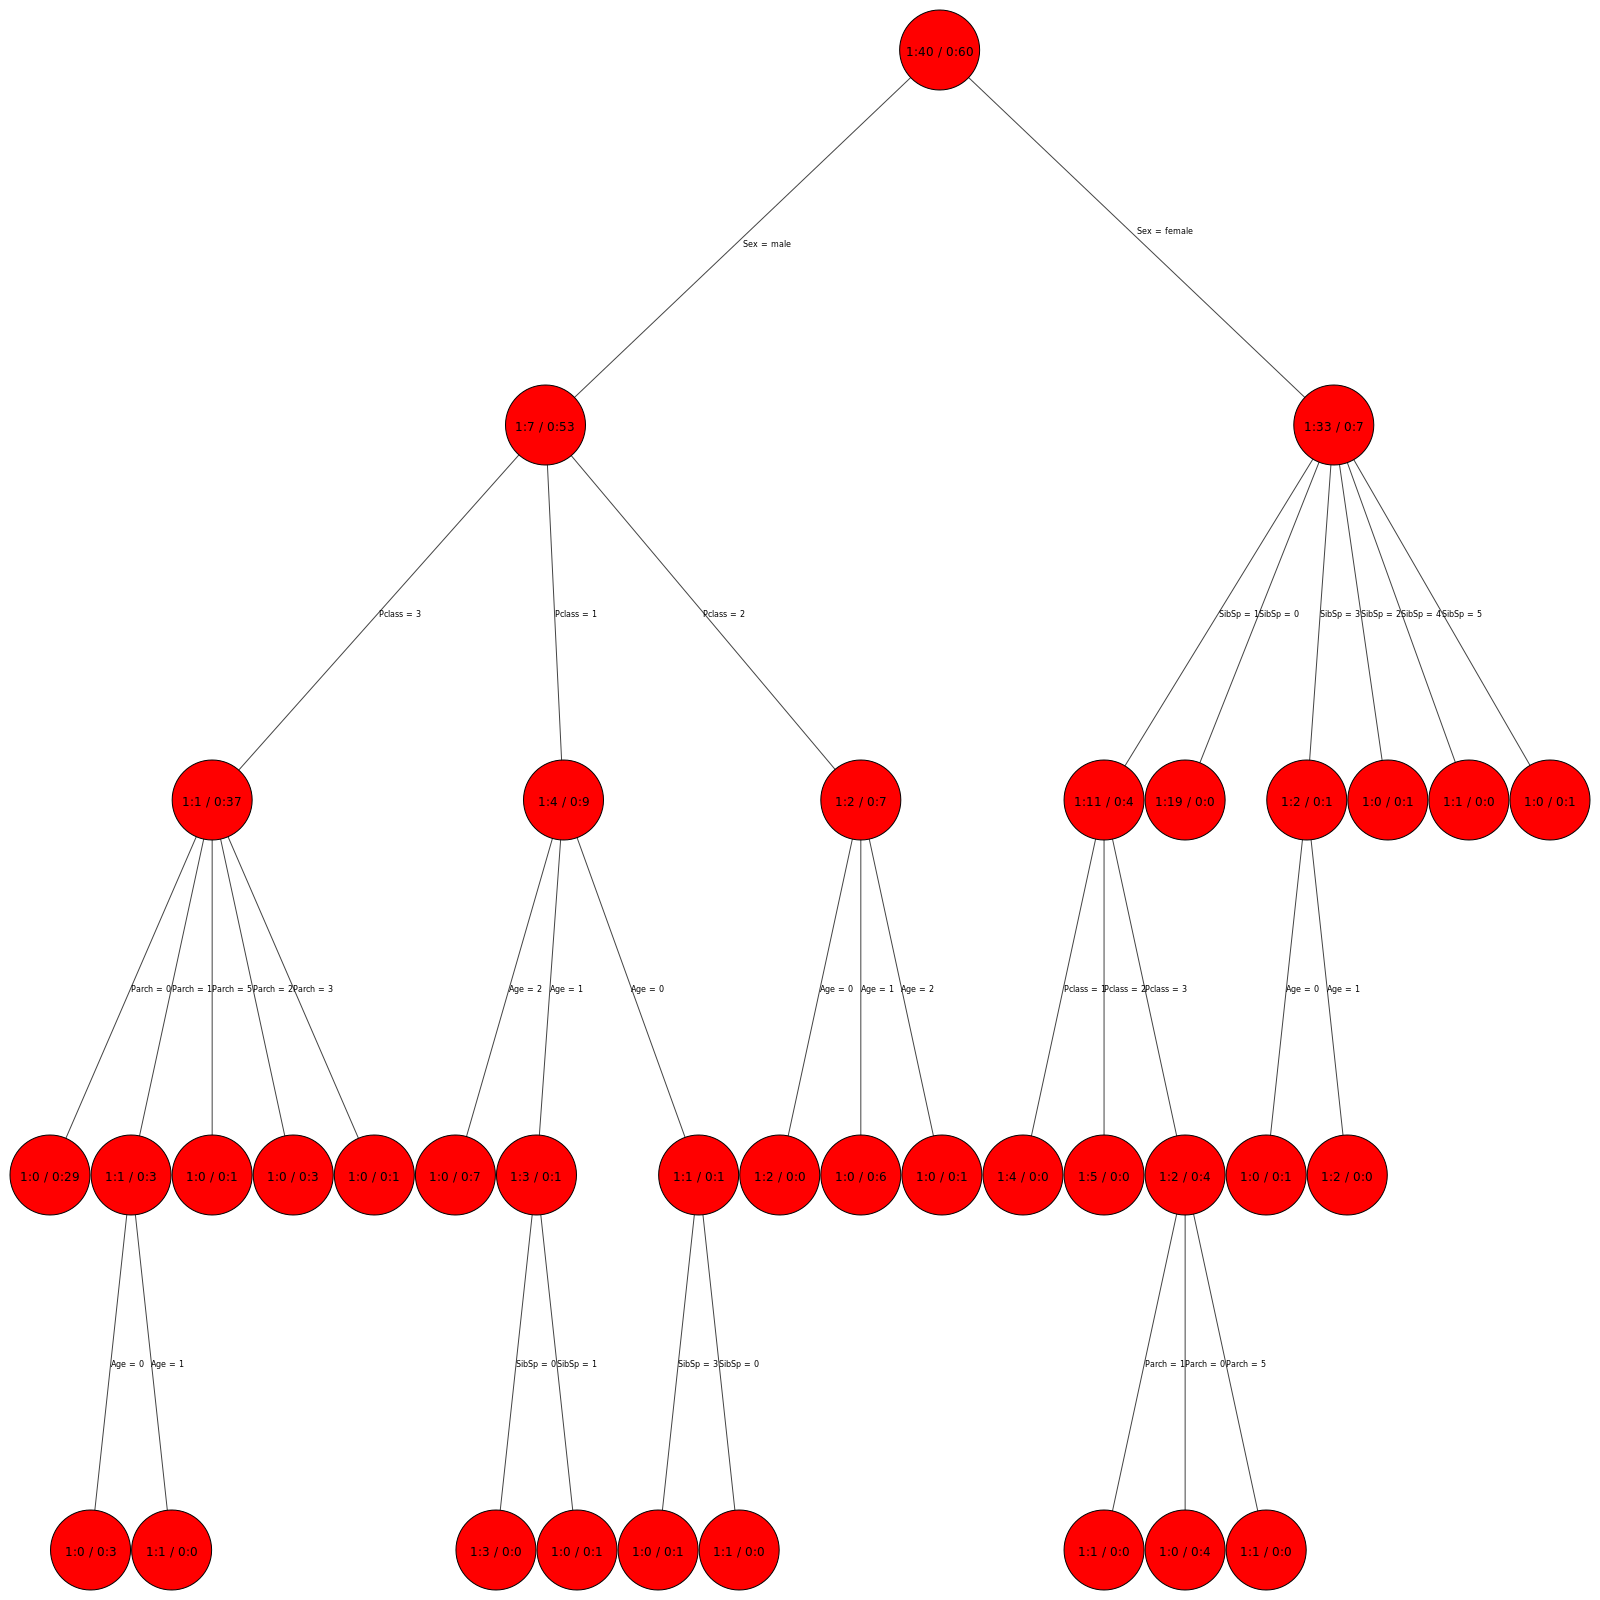
\includegraphics[width=\linewidth]{Ciagly.png}
	\end{subfigure}
	\label{fig:ciagle}
	\caption{Age jest atrybutem ciągłym}
\end{figure}

\end{document}
